\documentclass[10pt,a4paper]{article}

\usepackage[margin=0.5cm]{geometry}
\usepackage{multicol}
\usepackage{amsmath, amssymb}
\usepackage{tcolorbox}
\usepackage{enumitem}
\usepackage{makecell}
\usepackage{tabularx}
\usepackage{tikz}
\usepackage{pgfplots}
\pgfplotsset{compat=1.18} % latest stable

\usepackage{tikz}
\usepackage[utf8]{inputenc}
\usepackage[T1]{fontenc}
\usetikzlibrary{arrows.meta}

% compact lists
\setlist{nosep}

% compact sections
\setlength{\parindent}{0pt}
\setlength{\parskip}{0pt}

\begin{document}

\begin{center}
  \bfseries\Huge Questionario Socrative
\end{center}
\vspace{20pt}

1. Cuatro estaciones sondean un canal Ethernet sobre medio compartido y lo encuentran ocupado.
Suponiendo que todas van a experimentar la primera colisión, ¿cuál es la probabilidad de que una cualquiera de
ellas consiga transmitir con éxito en el primer intento?

\begin{enumerate}[label=\alph*]
    \item 0.25
    \item \textbf{0.50}
    \item 0.125
    \item 0.0625
    \item Todas las respuestas restantes son falsas.
\end{enumerate}

\textbf{Explicación}

La probabilidad de que una estación concreta transmita con éxito es la probabilidad de que dicha estación
elija un slot y las otras tres elijan el otro slot. Eso ocurre con probabilidad $2*0.5*0.5^3 = 2*0.5^4$
(la multiplicación por 2 es para tener en cuenta que hay dos formas de conseguir la transmisión en el primer
intento, es decir, transmitir con éxito en el primer slot o transmitir con éxito en el segundo slot).

Puesto que la estación concreta puede ser, en realidad, cualquiera de las cuatro, hay 4 formas de que se cumpla
la condición anterior, por lo que el resultado definitivo es $4*2*0.5^4 = 0.5$.

\vspace{15pt} \hrule \vspace{15pt}




2. Señalar cuál de las siguientes afirmaciones acerca de las redes Ethernet es correcta:

\begin{enumerate}[label=\alph*]
    \item En Ethernet sobre medio compartido, las colisiones se detectan por la no recepción de un ACK.
    \item \textbf{En Ethernet sobre medio compartido, las tramas colisionadas se retransmiten, y las no colisionadas, pero detectadas erróneas, se descartan.}
    \item En Ethernet conmutado, las tramas erróneas se retransmiten.
    \item En Ethernet sobre medio compartido y topología en estrella o árbol centrada en hub, el hub sólo repite las tramas que recibe correctamente.
    \item En Ethernet conmutado, las transmisiones son half-duplex.
\end{enumerate}
\textbf{Explicación}

En Ethernet, sólo hay retransmisión de tramas cuando es sobre medio compartido y se produce colisión de tramas.
En el resto de casos, las tramas se descartan sin retransmisión.

Un hub repite la trama que recibe por un puerto de entrada por los restantes puertos de salida, sea correcta o
no, pues este dispositivo no analiza el contenido de la misma.

En Ethernet conmutado, cada dispositivo final tiene un enlace punto a punto bidireccional y full-duplex con un
conmutador.

\vspace{15pt} \hrule \vspace{15pt}




3. Un computador conectado a una red Ethernet ejecuta una aplicación que hace uso del protocolo de transporte
TCP. Suponiendo que el direccionamiento es IPv6, ¿cuánto vale el parámetro MSS de la conexión?

\begin{enumerate}[label=\alph*]
    \item 1460 B.
    \item 1452 B.
    \item \textbf{1440 B.}
    \item 1472 B.
    \item 1466 B.
\end{enumerate}
\textbf{Explicación}

El valor MTU de Ethernet es 1500 B. Si le restamos los 40 B de cabecera IPv6 y los 20 B de cabecera TCP,
resulta un valor de MSS de 1440 B.

\vspace{15pt} \hrule \vspace{15pt}




4. ¿Cuánto vale la velocidad media disponible por estación en una red Ethernet 1000BASE-T que interconecta 20
estaciones, todas activas? Suponer tramas de tamaño máximo.

\begin{enumerate}[label=\alph*]
    \item \textbf{26.5 Mbps aprox.}
    \item 529.3 Mbps aprox.
    \item 45 Mbps aprox.
    \item 21.5 Mbps aprox.
    \item 6.2 Mbps aprox.
\end{enumerate}
\textbf{Explicación}

Ethernet 1000BASE-T es sobre medio compartido. Se trata de aplicar la fórmula de eficiencia con $N = 20$
estaciones y $\tau_b = 4096$ bits (duración equivalente en bits de los slots de contención).
Al multiplicar la eficiencia resultante por la velocidad nominal (1000 Mbps) y dividir por el total de estaciones,
se obtienen 26.5 Mbps aprox. por estación.

\vspace{15pt} \hrule \vspace{15pt}


\pagebreak

5. En una red Ethernet sobre medio compartido, 4 estaciones sondean el canal y lo encuentran ocupado.
Tras el primer slot de colisión inevitable, las 4 estaciones activan el algoritmo BEB con 2 slots
(primera etapa). ¿Cuál es la probabilidad de que las 4 estaciones tengan que ejecutar la segunda etapa del
algoritmo?

\begin{enumerate}[label=\alph*]
    \item 0.125.
    \item 0.375.
    \item 0.4375.
    \item 0.3125.
    \item \textbf{0.5}
\end{enumerate}
\textbf{Explicación}

La única forma de que se produzca una transmisión con éxito en la primera etapa es que una de las estaciones
elija un slot y las restantes elijan el otro slot. Si les damos nombre a las estaciones, por ejemplo,
A, B, C y D, y suponemos que es la estación A que transmite con éxito, la probabilidad de que eso ocurra es
$2*0.5*0.5^3$ (el 2 proviene de que A puede transmitir con éxito en el primer slot o en el segundo,
por lo que hay 2 opciones).

Como no tiene por qué ser A la que transmita con éxito, sino que puede ser
cualquiera de las 4 estaciones, multiplicamos el resultado anterior por 4: $4*2*0.5*0.5^3 = 0.5$.
La probabilidad solicitada es la complementaria de este valor, es decir, 0.5.

\vspace{15pt} \hrule \vspace{15pt}




\begin{multicols}{2}
    6. Dos dispositvos A y B intercambian datos mediante el protocolo de enlace HDLC.
    Después de transmitir la trama I-4-5, el tamaño actual de la ventana de transmisión de A se queda en 5.
    ¿Qué tramas de datos puede enviar A después de recibir la trama REJ4?
    
    \begin{enumerate}[label=\alph*]
        \item I-4-5, I-5-5, I-6-5, I-7-5.
        \item I-4-5, I-7-5, I-8-5, I-9-5.
        \item I-4-5, I-5-5, I-6-5, I-7-5, I-0-5, I-1-5.
        \item \textbf{I-4-5, I-5-5, I-6-5, I-7-5, I-8-5, I-9-5.}
        \item Las otras secuencias son incorrectas.
    \end{enumerate}
    \columnbreak
    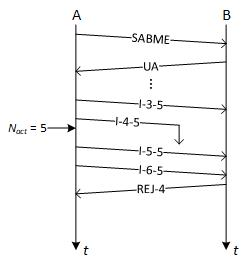
\includegraphics[width=0.5\textwidth]{1.jpeg}
\end{multicols}
\textbf{Explicación}

Los dos dispositivos acuerdan trabajar en formato extendido (SABME), por lo que el número de bits para
secuenciar las tramas es 7. La trama REJ4 es un rechazo no selectivo, es decir, se trata de un volver-atrás-N,
esta vez desde la trama I-4-5, lo que significa que el tamaño de la ventana del transmisor vuelve al estado en
que se hallaba antes de transmitir la trama I-4-5, es decir, vuelve a tener un valor 6.

Por tanto, puede transmitir 6 tramas desde la trama I-4-5 inclusive, teniendo además en cuenta que la
numeración permite superar el valor 7.

\vspace{15pt} \hrule \vspace{15pt}




\pagebreak

\begin{multicols}{2}
    7. Dos dispositivos dialogan de acuerdo con el protocolo HDLC en el modo ABM extendido. La trama de datos I-91-42 es la última que A envía y, como muestra el diagrama, se pierde. ¿Qué opción conducirá a la retransmisión de dicha trama lo más rápido posible?

    \begin{enumerate}[label=\alph*]
        \item La sola recepción de la trama I-42-91 ya indica a la estación A que debe retransmitir la trama I-91-42.
        \item La estación A tiene que esperar a que expire el temporizador de la trama I-91-42 (condición de timeout).
        \item \textbf{La estación A debería realizar un chekpoint tras recibir la trama I-42-91, enviando una trama RR-43-P.}
        \item La estación B debería enviar una trama REJ-91.
        \item Descartar la trama y que TCP se encargue de la retransmisión del segmento encapsulado en la misma.
    \end{enumerate}
    \columnbreak
    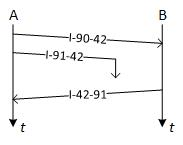
\includegraphics[width=0.5\textwidth]{2.jpeg}
\end{multicols}
\textbf{Explicación}

La recepción de la trama I-42-91 sólo indica que el receptor ya ha procesado la trama I-90-42, no que la trama
I-91-42 se haya perdido.  Puesto que se ha perdido y es la última, B no puede saber que A envió la trama
I-91-42 y, por ello, no puede enviar un REJ-91. Esperar el vencimiento del temporizador retrasaría mucho la
retransmisión, por lo que la alternativa mejor es que A realice un checkpoint.

\vspace{15pt} \hrule \vspace{15pt}




8. Señalar la afirmación correcta acerca del protocolo HDLC:

\begin{enumerate}[label=\alph*]
    \item El estándar incluye la especificación de capa física.
    \item Sólo puede utilizarse en enlaces punto a punto.
    \item Puesto que implementa las funciones de control de flujo y errores, puede utilizarse tanto en la capa de enlace como en la capa de transporte.
    \item \textbf{HDLC proporciona un servicio orientado a la conexión.}
    \item Para transmisiones a larga distancia, es mejor configurar HDLC con 3 bits de secuenciación (formato normal).
\end{enumerate}
\textbf{Explicación}

HDLC proporciona un servicio orientado a la conexión, pues al principio ésta debe establecerse para fijar el
modo de operación (ABM, NRM o ARM) y el uso o no del formato extendido. Las demás opciones son claramente
falsas.

\end{document}